\documentclass[letterpaper,11pt]{article}

\usepackage[margin=1in]{geometry}
\usepackage[titletoc,title]{appendix}
\usepackage{amsmath}
\usepackage{amssymb}
\usepackage{amsthm}
\usepackage{amscd}
\usepackage{amsfonts}
\usepackage{graphicx}%
\usepackage{fancyhdr}
\usepackage{color}
\usepackage{sectsty}
\usepackage[colorlinks=true,linkcolor=black,anchorcolor=black,citecolor=black,filecolor=black,menucolor=black,runcolor=black,urlcolor=black]{hyperref}
\usepackage{siunitx}
\usepackage{cleveref}
% \usepackage{natbib}
% \usepackage{biblatex} %Imports biblatex package
% \addbibresource{PDR.bib} %Import the bibliography file
\usepackage{csquotes}
\usepackage{array}
\usepackage{tablefootnote}
\usepackage[]{todonotes}

%-----------------------------------------------

\hyphenation{LArTPC}
\hyphenation{LArTPCs}

\newcommand{\tslarpaas}      {t_{\text{SLArPAAS I}}}
\newcommand{\davg}           {d_{\text{avg}}}

%---------------------------------------------

\renewcommand{\arraystretch}{1.2}

%-----------------------------------------------

\pagestyle{fancy}\lhead{}
\setlength{\parindent}{0em}

\title{SLArpaas Pressure Test Plan}
\author{Yun-Tse Tsai}

%-----------------------------------------------

\begin{document}

\maketitle
\tableofcontents

%------------------------------------------------
% Main text
% -----------------------------------------------

\section{P\&ID and boundary limits of test}

Fig.~\ref{fig:PID} shows the P\&ID of the whole liquid argon system, 
while the yellow dashed line defines the boundary limits of this
pressure test.

% ----------------------------------------------------------
\begin{figure}[h]
    \centering
    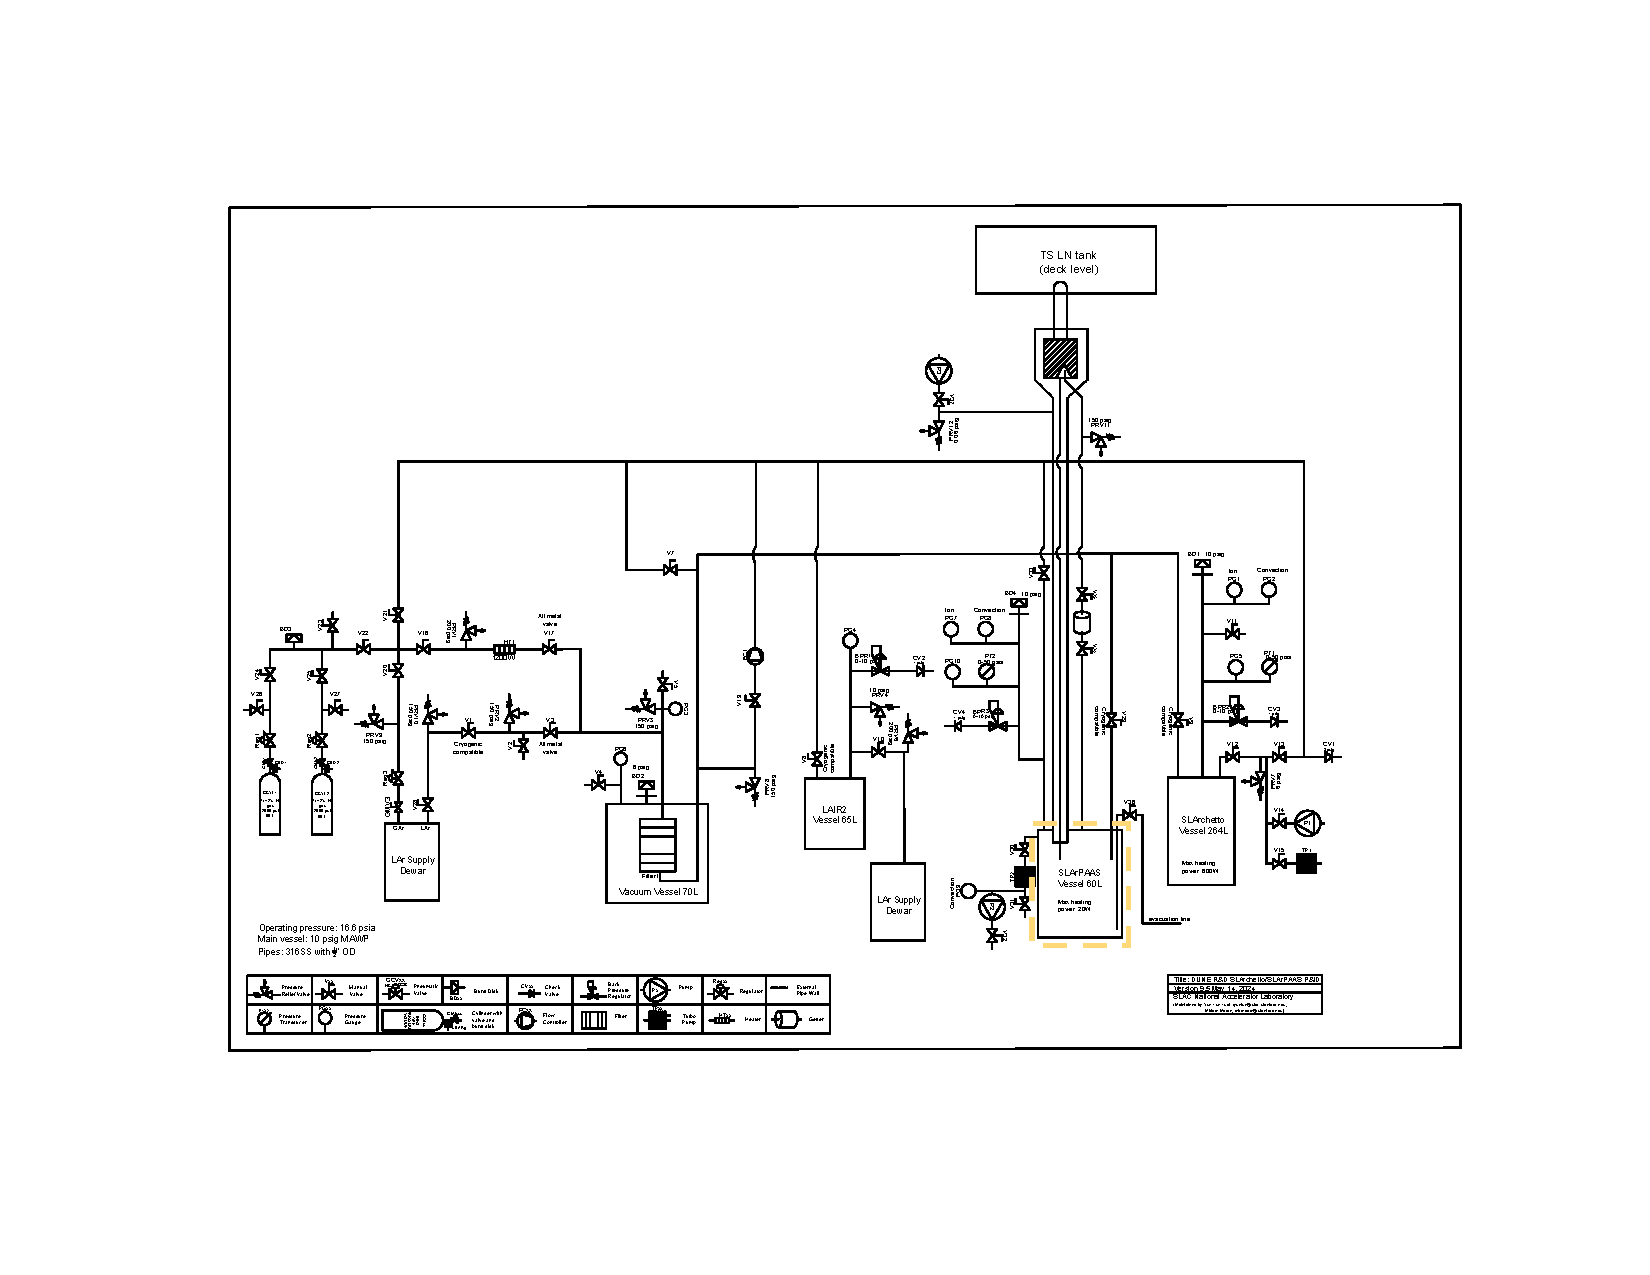
\includegraphics[width=\textwidth]{fig/PID_SLArchettoPAAS_v9.5_PressureTest.pdf}
    \caption{P\&ID of the LAr setups at LNTF.  The yellow dashed line defines the boundary
    limits of this pressure test, the SLArPAAS I vessel and top plate.}
    \label{fig:PID}
\end{figure}
% ----------------------------------------------------------

%------------------------------------------------
\section{Pressure test schematic diagram}

Fig.~\ref{fig:PressureTest_PID} shows the schematic diagram of this pressure test.

% ----------------------------------------------------------
\begin{figure}[h]
    \centering
    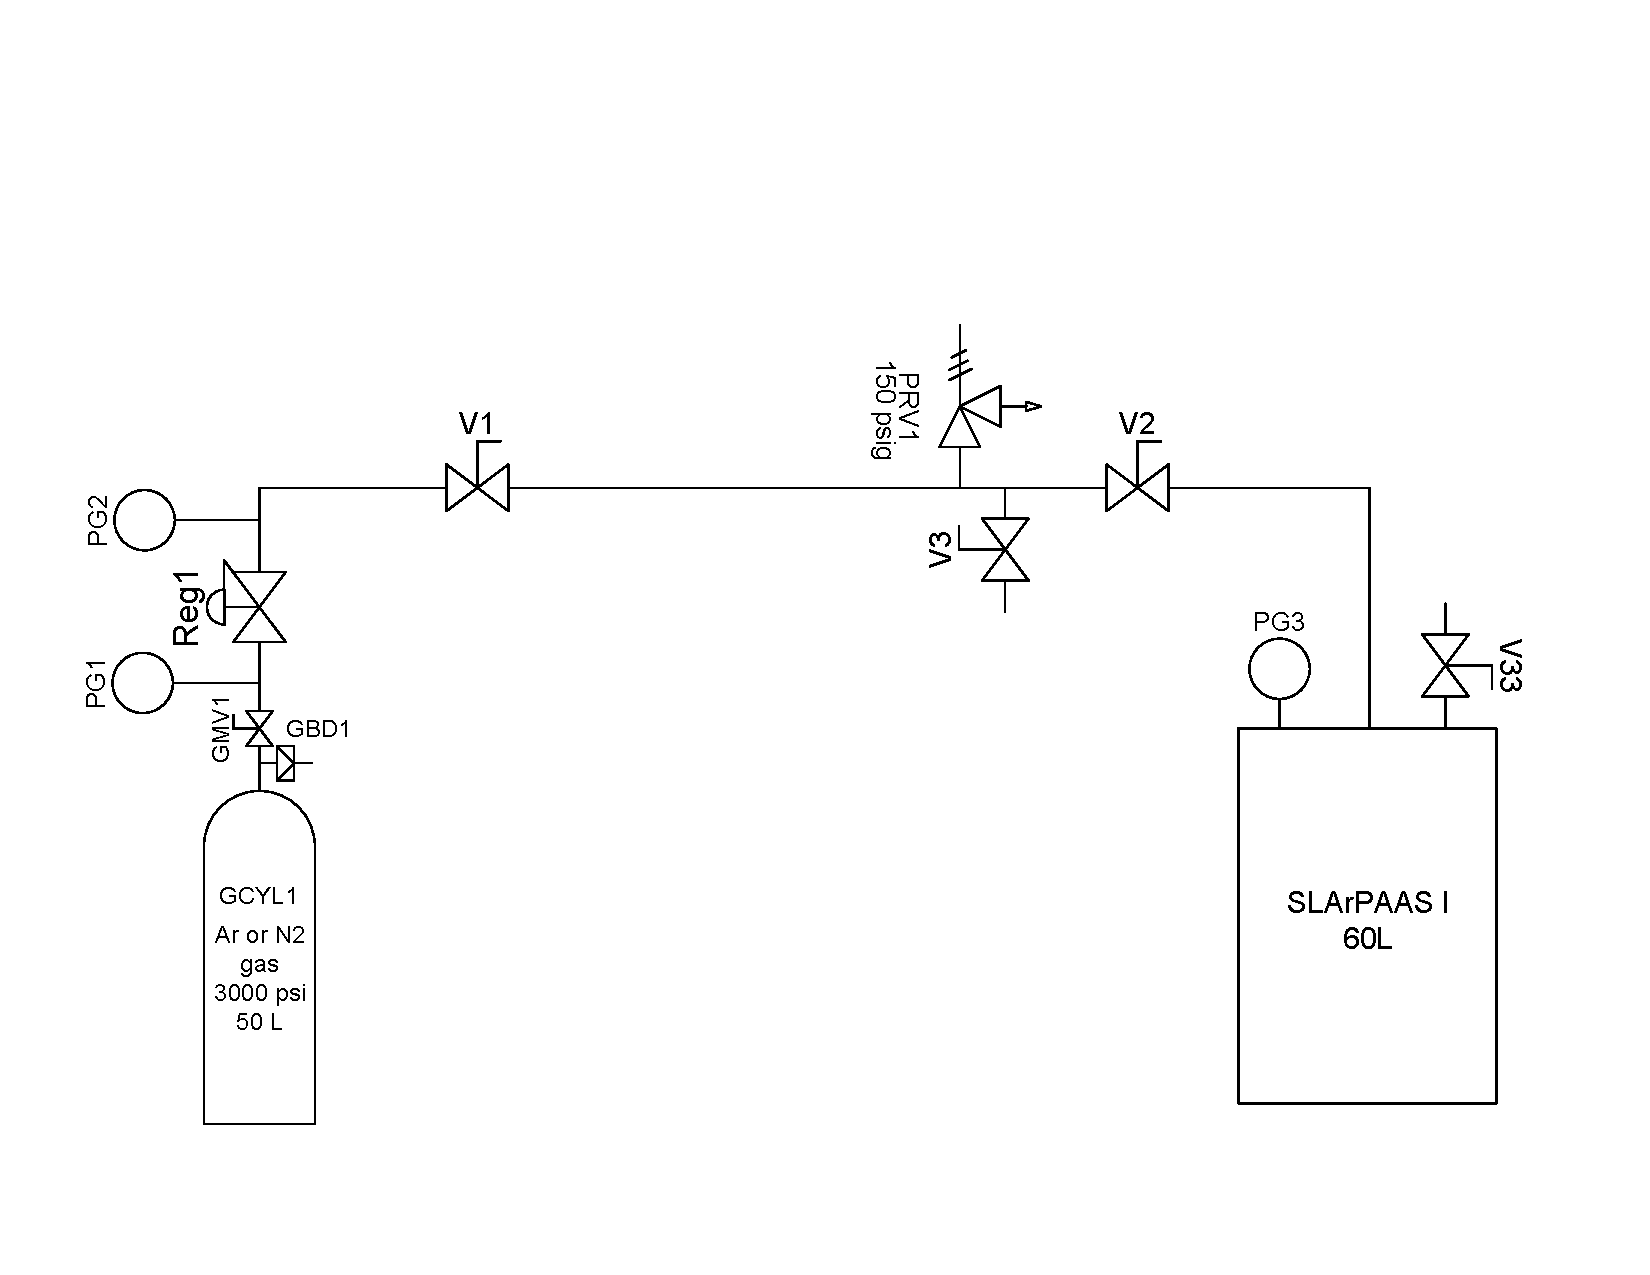
\includegraphics[width=\textwidth]{drawing/PressureTestPID-Model.pdf}
    \caption{Schematic diagram of this pressure test.}
    \label{fig:PressureTest_PID}
\end{figure}
% ----------------------------------------------------------

%------------------------------------------------
\section{Project technical specifications}

The engineering note of SLArPAAS I can be found at \\
\url{https://drive.google.com/file/d/1v5ZKb8rsPxWNhKpIrJMqwthE9KjeZ3Yi/view?usp=sharing}.

%------------------------------------------------
\section{Pressure test procedures}

\begin{enumerate}
    \item Connect the SLArPAAS I dewar to the argon (or nitrogen) cylinder, GCYL1, 
    as shown in Fig.~\ref{fig:PressureTest_PID}. All valves should be at close position.
    \item Use signages and caution tapes to secure the exclusive area, the LNTF hut and behind.
    \item Keep V1 and V3 at close position, open GCYL1 (valve GMV1), increase the deliver pressure (PG2)
    from the regulator gradually to about 6~psig.
    \item Open V1.
    \item Keep V33 closed and open V2. The PG3 pressure should increase. Pay attention to any hissing
    sound. A hissing usually indicates a leak. If there is hissing sound, check and fix the problem.
    \item Monitor the pressure of PG3. When there is no decrease in pressure, adjust the pressure
    regulator so that PG3 is at 12.5~psig.
    \item Close both V1 and V2. Monitor PG3 over one hour. If the pressure change is
    less than 0.5~psi and there is no visual deformation observed at the dewar from the pressure test, 
    the pressure test is satisfied.
    Note: Pressure maybe slightly change initially due to the expansion of the test gas.
\end{enumerate}

%------------------------------------------------
\textbf{Return to the Original Configuration}

\begin{enumerate}
    \item Close GMV1 at the gas cylinder GCYL1 and open V3.
    \item Open V2. Now the argon or nitrogen gas at the dewar vents.
    Note: the minimum room size to dilute the nitrogen or argon gas from becoming an asphyxiant 
    is 3.2~m$^3$ calculated per ASHRAE 34, which is much smaller than the room volume where the dewar 
    or the test gas cylinder locates.
    \item When PG3 reads zero, close V2 then disconnect the flexible line connection from V2.
    \item Disconnect the piping on the argon (or nitrogen) gas cylinder, GCYL1.
    \item Remove PG3.
    \item Remove the signages and caution tapes.
    \item Install the burst disc back in place.
    \item Install the BPR3 and CV4 back in place.
\end{enumerate}

%------------------------------------------------
\section{Gauge calibration document}

PG3 used in the pressure test has the range of 0 to 30~psi, as listed in
\url{https://www.mcmaster.com/9796T31/}.
It has the calibration certificate traceable to NIST, as shown in Fig.~\ref{fig:PG3Certificate} below.
(will be updated when receiving the gauge.)


% ----------------------------------------------------------
\begin{figure}[h]
    \centering
    % \includegraphics[width=\textwidth]{}
    \caption{}
    \label{fig:PG3Certificate}
\end{figure}
% ----------------------------------------------------------

%------------------------------------------------
% Appendix
% -----------------------------------------------
% \clearpage
% \begin{appendices}

% \clearpage    
% \end{appendices}

\end{document}